\documentclass[10pt,a4paper]{article}

%double si on veut une version prof et une version élève. simple si on veut une seule version.
\newcommand{\buildmode}{double}

\InputIfFileExists{version.tex}{}{}
% Version (définie par le script)
\providecommand{\version}{eleve}

\usepackage{../../feuilleexo}

%%%à modifier à chaque fois

\renewcommand{\niveau}{2nde}
\renewcommand{\chapitre}{Proportions}
\renewcommand{\numchap}{1}
\renewcommand{\theme}{Proportions}

\begin{document}

\montitre{Fiche d'exercices : \chapitre}

\vspace{-0.3cm}

\begin{prerequis}[Capacités attendues]
\begin{itemize}
    \item Exploiter la relation entre effectifs, proportions et pourcentages.
    \item Traiter des situations simples mettant en jeu des pourcentages de pourcentages.
\end{itemize}
\end{prerequis}
\begin{multicols}{2}


\section{Sans calculatrice}

\begin{exo}
À la rentrée 2023, en Ligue 1 de football, il y a 9 entraineurs français sur un total de 18 entraineurs de club. Quelle proportion d'entraineurs français y a-t-il en Ligue 1 de football ?
\end{exo}

\begin{exo}
Un commerçant souhaite vendre un chocolat chaud à 3€ hors taxes. La taxe sur la valeur ajoutée (TVA) pour les boissons non alcoolisées est de $10\%$. Combien vaut le chocolat chaud avec la TVA ? Peut-on dire que lorsque je paie mon chocolat chaud, je paie 10\% de TVA ?
\end{exo}

\begin{exo}[QCM]
Pour chacune des questions de ce questionnaire à choix multiples, une seule réponse est exacte.

\medskip

\begin{enumerate}[leftmargin=*]
    \item Parmi les 1057 élèves du lycée GT, 333 sont en seconde. Quel est le pourcentage d'élèves en seconde ?
    \begin{tasks}(3)
        \task $10,3\%$
        \task $31,5\%$
        \task $49,1\%$
    \end{tasks}

    \item En 2015, la ville de Saint-Denis comptait 111 103 habitants, parmi lesquels $51,86\%$ environ vivaient dans les quartiers \og La Plaine \fg{}, \og Grand centre-ville \fg{} et \og Franc-Moisin - Bel Air - Stade de France \fg{}. Quel est le nombre d'habitants qui vivaient dans ces quartiers en 2015 ? (Source : \textit{INSEE})
    \begin{tasks}(3)
        \task 26 343
        \task 52 503
        \task 57 615
    \end{tasks}
\end{enumerate}
\end{exo}

\section{Avec calculatrice}

\begin{minipage}{0.5\textwidth}
\begin{exo}
À l'aide de l'illustration ci-contre, répondre aux questions suivantes :
\begin{enumerate}[leftmargin=*]
    \item Quelle est la proportion de lycées polyvalents parmi les lycées de l'académie ?
    \item Quelle est la part des personnels qui n'est pas enseignant ?
    \item Dans l'académie de Créteil, y a-t-il plus de lycées professionnels dans le public ou le privé ?
\end{enumerate}
\end{exo}

\begin{exo}
Pour une personne seule, gagnant moins de 27 478€ par an, l'impôt sur le revenu fonctionne de la manière suivante :
\begin{itemize}
    \item Les premiers 10 777€ sont imposés à $0\%$.
    \item De 10 778€ à 27 478€, le taux d'imposition est de $11\%$.
\end{itemize}
Combien paiera d'impôts une personne ayant gagné 8 000€ dans l'année ? Et une personne ayant gagné 25 000€ ?
\end{exo}
\end{minipage}
\hfill
\begin{minipage}{0.45\textwidth}
    \centering
    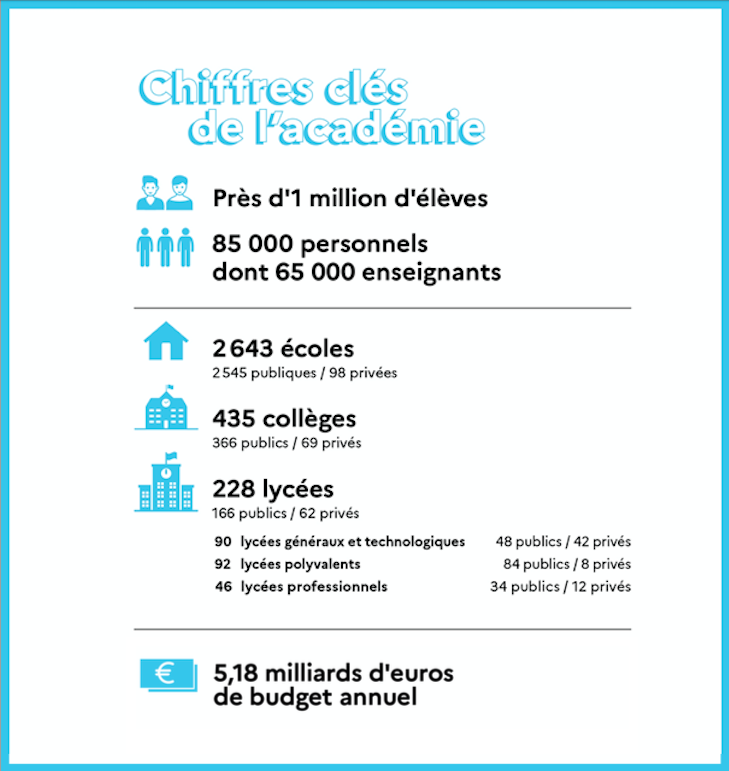
\includegraphics[width=\textwidth]{2NDE_Chapitre_1_Exo___Proportions/chiffres-aca.png}

    \footnotesize Source : rectorat de Créteil
\end{minipage}

\begin{exo}
En France métropolitaine, sur le troisième trimestre 2018, le taux de chômage correspond à $8\%$ de la population active. On compte $2,6$ millions de chômeurs. À combien s'élève la population active à cette date ?
\end{exo}

\begin{exo}
D'après l'étude \textit{The Global Human Day} du PNAS, les humains passent en moyenne 9h 6min par jour à dormir. Quelle proportion du temps passent-ils éveillés, en moyenne ?
\end{exo}

\begin{exo}
L'algorithme ci-dessous permet de retrouver le résultat de l'exercice sur la TVA du chocolat chaud. Réécrire l'algorithme pour qu'il calcule le prix TTC d'un café à $1,50$€.

\begin{leftbar}
$a \leftarrow 0,1$

$b \leftarrow 3$

$c \leftarrow a \times b$

$d \leftarrow b + c$
\end{leftbar}
\end{exo}

\begin{exo}
Trois amis A, B et C décident de faire un repas commun. A apporte 5 plats ; B en apporte 3. C n'apporte rien, mais dit qu'il remboursera ses amis. En supposant que tous les plats ont la même valeur, C verse en accord avec les autres 16€. Comment répartir cette somme équitablement ?
\end{exo}

\begin{exo}
Au lycée, $31,5\%$ des élèves sont en filière technologique, parmi lesquels $25,5\%$ sont en section STI2D. Quelle est la proportion d'élèves en STI2D au lycée ?
\end{exo}

\begin{exo}
D'après les statistiques de l'Insee, la France comptera 74 millions d'habitants en 2050. Parmi les Français, les personnes de plus de 65 ans représenteront $40\%$. De plus, $60\%$ des plus de 65 ans auront plus de 75 ans. Quelle sera la proportion de Français âgés de plus de 75 ans en 2050 ? Donner le résultat en pourcentage.
\end{exo}

\begin{minipage}{0.6\textwidth}
\begin{exo}[Vrai ou faux]
Les affirmations suivantes sont-elles vraies ou fausses ? Justifier, sans calculatrice :
\begin{enumerate}[leftmargin=*]
    \item \textit{Affirmation :} Pour calculer la superficie des territoires indigènes (voir illustration ci-contre) en région amazonienne, on effectue le calcul $\displaystyle 8\,470\,209 \times \frac{28,6}{100}$.
    \item La part des filles choisissant l'enseignement de spécialité mathématiques en première générale est de $61,4\%$ (source : MENJ-DEPP).

    \textit{Affirmation :} On peut en déduire que la part de garçons choisissant l'enseignement de spécialité mathématiques est de $38,7\%$.
    \item Dans la recette du quatre-quart, il faut mettre un quart de beurre, un quart de sucre, un quart de farine et un quart d'oeufs.

    \textit{Affirmation :} Si je rajoute à la recette d'origine 60g de beurre, de sucre, de farine, et d'oeuf, le gâteau est toujours un quatre-quart.
    \item \textit{Affirmation :} 70\% de 40\% c'est la même chose que 40\% de 70\%.
\end{enumerate}
\end{exo}
\end{minipage}
\hfill
\begin{minipage}{0.37\textwidth}
    \centering
    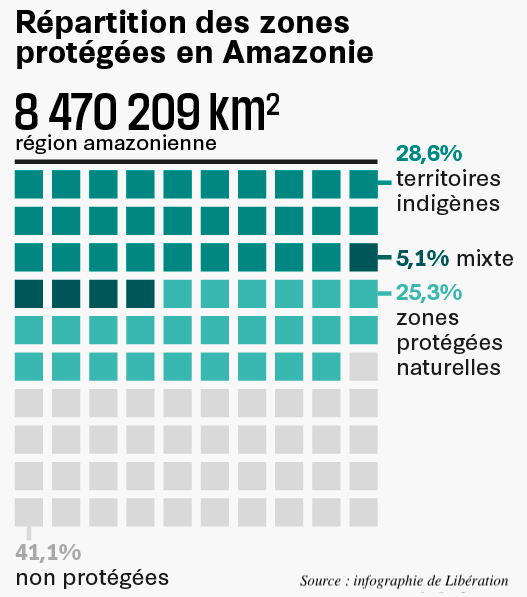
\includegraphics[width=.95\textwidth]{2NDE_Chapitre_1_Exo___Proportions/foret-amazonienne.png}

    \footnotesize Extrait d'une infographie du journal \textit{Libération} : \og La perte du couvert forestier en Amazonie \fg{}
\end{minipage}

\end{multicols}

\end{document}
